% #######################################
% ########### FILL THESE IN #############
% #######################################
\def\mytitle{CONIC ASSIGNMENT}
\def\mykeywords{}
\def\myauthor{SIVA PARVATHI TUNGALA}
\def\contact{tvssn143@gmail.com}
\def\mymodule{ Future Wireless Communication(FWC22089)}
% #######################################
% #### YOU DON'T NEED TO TOUCH BELOW ####
% #######################################
\newcommand{\myvec}[1]{\ensuremath{\begin{pmatrix}#1\end{pmatrix}}}
\let\vec\mathbf
\providecommand{\pr}[1]{\ensuremath{\Pr\left(#1\right)}}
\providecommand{\qfunc}[1]{\ensuremath{Q\left(#1\right)}}
\providecommand{\sbrak}[1]{\ensuremath{{}\left[#1\right]}}
\providecommand{\lsbrak}[1]{\ensuremath{{}\left[#1\right.}}
\providecommand{\rsbrak}[1]{\ensuremath{{}\left.#1\right]}}
\providecommand{\brak}[1]{\ensuremath{\left(#1\right)}}
\providecommand{\lbrak}[1]{\ensuremath{\left(#1\right.}}
\providecommand{\rbrak}[1]{\ensuremath{\left.#1\right)}}
\providecommand{\cbrak}[1]{\ensuremath{\left\{#1\right\}}}
\providecommand{\lcbrak}[1]{\ensuremath{\left\{#1\right.}}
\providecommand{\rcbrak}[1]{\ensuremath{\left.#1\right\}}}
\documentclass[10pt, a4paper]{article}
\usepackage[a4paper,outer=1.5cm,inner=1.5cm,top=1.75cm,bottom=1.5cm]{geometry}
\twocolumn
\usepackage{circuitikz}
\usepackage{amsmath,bm}
\usepackage{amsthm}
\usepackage{mathtools}
\usepackage{amsfonts}
\usepackage{amssymb}
\usepackage{graphicx}
\usepackage{bm}
\newcommand{\bfitDelta}{\bm{\mathit{\Delta}}}

\graphicspath{{./images/}}
%colour our links, remove weird boxes
\usepackage[colorlinks,linkcolor={black},citecolor={blue!80!black},urlcolor={blue!80!black}]{hyperref}
%Stop indentation on new paragraphs
\usepackage[parfill]{parskip}
%% Arial-like font
\usepackage{lmodern}
\renewcommand*\familydefault{\sfdefault}
%Napier logo top right
\usepackage{watermark}
%Lorem Ipusm dolor please don't leave any in you final report ;)
\usepackage{karnaugh-map} 
\usepackage{tabularx}
\usepackage{lipsum}
\usepackage{xcolor}
\usepackage{listings}
%give us the Capital H that we all know and love
\usepackage{float}
%tone down the line spacing after section titles
\usepackage{titlesec}
%Cool maths printing
\usepackage{amsmath}
%PseudoCode
\usepackage{algorithm2e}

\titlespacing{\subsection}{0pt}{\parskip}{-3pt}
\titlespacing{\subsubsection}{0pt}{\parskip}{-\parskip}
\titlespacing{\paragraph}{0pt}{\parskip}{\parskip}
\newcommand{\figuremacro}[5]{
    \begin{figure}[#1]
        \centering
        \includegraphics[width=#5\columnwidth]{#2}
        \caption[#3]{\textbf{#3}#4}
        \label{fig:#2}
    \end{figure}
}


 \lstset{
frame=single, 
breaklines=true,
columns=fullflexible
}
\thiswatermark{\centering \put(1,-110){
\includegraphics[scale=0.05]{iitlogo.jpg}} }
\title{\mytitle}
\author{\myauthor\hspace{1em}\\\contact\\IITH\hspace{0.5em}-\hspace{0.5em}\mymodule}
\date{}
\hypersetup{pdfauthor=\myauthor,pdftitle=\mytitle,pdfkeywords=\mykeywords}
\sloppy
% #######################################
% ########### START FROM HERE ###########
% #######################################
\begin{document}
 \maketitle
 \tableofcontents
 
 \Large\section{Problem}
 Q.The locus of the mid-point of the lines segment joining the focus to a moving point on the parabola $y^2$=4a$x$ is another parabola with directrix
 
 \section{Solution}
The standard conic equation is,\\
\begin{align}
\textbf{x}^\top\textbf{Vx}+2\textbf{u}^\top\textbf{x}+f=0
\end{align} 
\raggedright where,\\
\centering
$\textbf{V}=\myvec{0&0 \\0&1}$\\ $\textbf{u}=\myvec{-2a\\0}$ and $f=0$ \\
\raggedright
let moving point on the parabola be 'q',then the equation is,
\begin{align}
\textbf{q}^\top\textbf{Vq}+2\textbf{u}^\top\textbf{q}+f=0
\end{align}
\raggedright
the mid-point when line segment joining the focus to moving point on the parabola be 'h'.
\begin{align}
\textbf{h}=\frac{\textbf{q+F}}{2}\\
\textbf{q}=2\textbf{h}-\textbf{F}
\end{align}
Substitube eq(4) in eq(2)\\
\begin{align}
(2\textbf{h}-\textbf{F})^\top\textbf{V}(2\textbf{h}-\textbf{F})+2\textbf{u}^\top(2\textbf{h}-\textbf{F})+f=0
\end{align}
By solving we get the locus parabola equation is, \\
\begin{align}
\textbf{x}^\top\textbf{V}_{1}\textbf{x}+2\textbf{u}_{1}^\top\textbf{x}+f_1=0
\end{align} 
where,\\
\centering
$\textbf{V}_{1}=\myvec{0&0 \\0&1}$\\ $\textbf{u}_{1}=\myvec{-a\\0}$ and $f_1=a^2$ \\
\raggedright
The directrix of a conic is given by,
\begin{align}
\textbf{n}^\top\textbf{x}=c
\end{align}
The directrices of eq(6) is given by,\\
\begin{align}
\textbf{n}=\sqrt{\lambda_2}\textbf{p}_{1}\\
c=\frac{\|\textbf{u}\|^2-\lambda_2 f}{2\textbf{u}^\top\textbf{n}} , \hspace{0.4cm} e=1
\end{align}
where the eigen values and eigen vectors are,\\
\begin{align}
\lambda_1=0 ,\hspace{0.3cm} \lambda_2=1\\
\textbf{p}_{1}=\myvec{1\\0},\hspace{0.3cm} \textbf{p}_{2}=\myvec{0\\1} 
\end{align}
substituting values in eq(8) we get,\\
\centering
\begin{align}
\textbf{n}=\myvec{1\\0}
\end{align}
\raggedright
substituting values in eq(9),\\
\centering
\vspace{2mm}
$c=\frac{a^2-a^2}{2\myvec{-a & 0}\myvec{1\\0}}$\\
\begin{align}
c=0
\end{align}
\raggedright
put n and c in directrix equation we get,
\centering
\begin{align}
\myvec{1&0}\textbf{x}=0
\end{align}
\raggedright
        Therefore,the locus of the mid-point of the lines segment joining the focus to a moving point on the parabola $y^2$-$4ax=0$ is another parabola $y^2$-$2ax$+$a^2=0$ with directrix $x=0$.\\
   \section{Plot}
\begin{figure}
       \centering
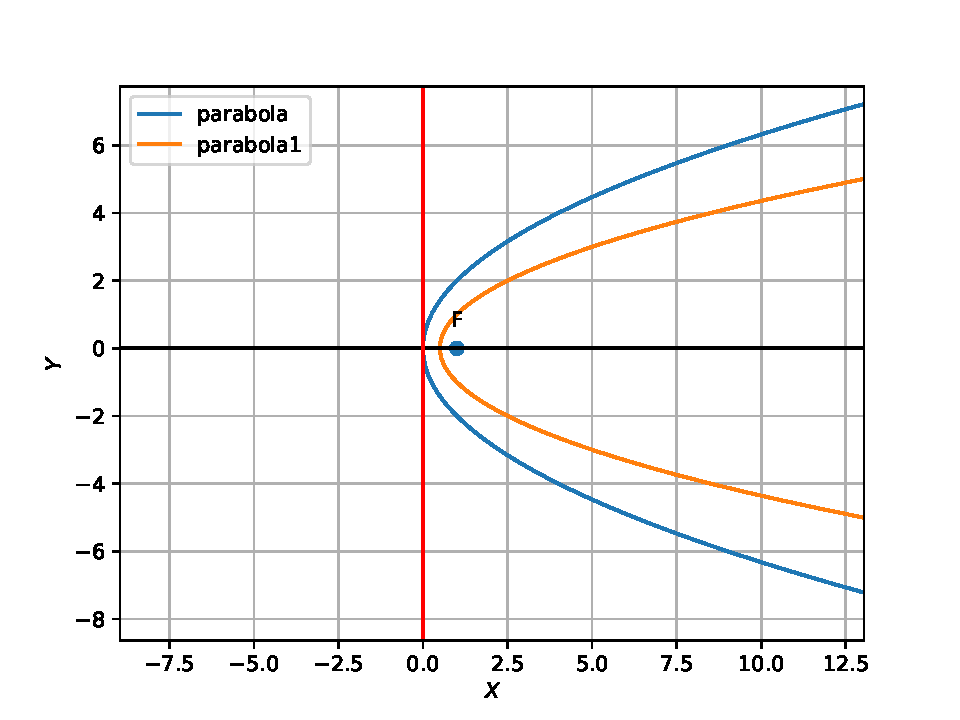
\includegraphics[width=\columnwidth]{cofig.pdf}
       \label{fig:my_label}
\end{figure}
\section{Software}
\raggedright
  We can get the parallel equation of given equation and the plot of two equtions by executing the following code:
 \vspace{1mm} 
\begin{lstlisting}
https://github.com/sivaparvathi-tungala/fwc_module_1/tree/main/conic
\end{lstlisting}
\end{document}\